\documentclass[11pt,a4paper]{article}
\usepackage[T1]{fontenc}
\usepackage[utf8]{inputenc}
\usepackage{lmodern,microtype,amsmath,amssymb,amsthm,mathtools}
\usepackage[margin=25mm,headheight=14pt]{geometry}
\usepackage{graphicx,booktabs,longtable,tabularx,array,enumitem,xcolor}
\usepackage{fancyhdr,listings,placeins,xurl}
\usepackage[colorlinks=true,linkcolor=blue!45!black,citecolor=blue!45!black,urlcolor=blue!55!black]{hyperref}
\usepackage[nameinlink,noabbrev]{cleveref}
\newtheorem{theorem}{Theorem}[section]
\newtheorem{lemma}[theorem]{Lemma}
\newtheorem{proposition}[theorem]{Proposition}
\newtheorem{corollary}[theorem]{Corollary}
\theoremstyle{definition}
\newtheorem{definition}[theorem]{Definition}
\theoremstyle{remark}
\newtheorem{remark}[theorem]{Remark}
\newcommand{\code}[1]{\texttt{#1}}
\newcommand{\Z}{\mathbb Z}
\newcommand{\F}{\mathbb F}
\newcommand{\NN}{\mathbb N}
\newcommand{\bits}{\operatorname{bits}}
\newcommand{\poly}{\operatorname{poly}}
\newcommand{\commit}{\texttt{9feb4346b4d050b305f825f0f7257f495960822a}}
\newcolumntype{Y}{>{\raggedright\arraybackslash}X}
\setlist{itemsep=3pt,topsep=5pt}
\setlength{\parskip}{2pt}
\setlength{\emergencystretch}{1.5em}
\pagestyle{fancy}
\fancyhf{}
\fancyhead[L]{\small ProveIt: compressed topology and elimination}
\fancyhead[R]{\small Research continuation, 9 October 2026}
\fancyfoot[C]{\thepage}
\lstset{basicstyle=\ttfamily\footnotesize,breaklines=true,columns=fullflexible,
  keepspaces=true,frame=single,rulecolor=\color{black!20},xleftmargin=0.5em,
  xrightmargin=0.5em,showstringspaces=false}
\graphicspath{{figures/}}
% Generated from retained results; do not edit measured JSON.
\newcommand{\FullTests}{1,044}
\newcommand{\LargestCertificateBytes}{1,259,441}

\hypersetup{pdftitle={Weighted Component Extraction and Persistent Elimination},
  pdfauthor={Research continuation for the ProveIt project},
  pdfsubject={Exact polynomial primitives towards quasi-polynomial unknot recognition}}

\title{\textbf{Weighted Component Extraction\\and Persistent Elimination}\\[0.6em]
  \large Exact polynomial primitives towards\\quasi-polynomial unknot recognition}
\author{Research continuation for Vladimir Reshetnikov's ProveIt project\\
  \small AI-assisted mathematical analysis, implementation, and independent audits}
\date{9 October 2026\\\small Baseline: \commit}

\begin{document}
\maketitle
\thispagestyle{empty}
\begin{abstract}
The ProveIt recognizer already contains exact compressed-word operations,
binary interval-orbit counting, independent local orbit proofs, and a
portfolio of knot simplification and decision procedures. Its remaining
asymptotic obstacles are global: finding useful transformations, controlling
the number of attempted transformations, and keeping every intermediate
encoding small. This continuation develops two complementary improvements.

First, a weighted observer on the maintained interval proof computes all
connected-component normal-coordinate vectors of a supplied surface,
with binary multiplicities. This makes the classical weighted
Agol--Hass--Thurston construction executable in the current code base,
replaces dense many-port subset enumeration by sparse incidence, and
extracts compressing disks from disconnected input surfaces. We prove a
sharp three-run increase for the actual suffix-transfer schedule and an
elementary support-sensitive bound: a surface with $v$ triangulation
vertices and $q$ active quadrilateral coordinates has at most $v+2q$
distinct component vectors, or $v+q$ when all components are two-sided.

Second, a signed persistent circuit represents an entire block of $k$ raw
singleton Tietze eliminations with
$O(S_0+k^2(D_0+1)+k^3\log(D_0+k+2))$ vertices, where $S_0$ and $D_0$
are the initial circuit size and concatenation depth. A final export to
an ordinary straight-line program at most doubles that size.

The accompanying code, tests, complete measurement samples, source hashes,
and independent component audits make these claims reviewable. The results
are polynomial primitives and a restricted representation theorem. They
do not establish a general quasi-polynomial bound for unknot recognition.
We state the missing composition hypotheses explicitly and propose a
prioritized research programme for resolving them.
\end{abstract}

\vfill
\noindent\small\textbf{Reading guide.} The main mathematical additions are the
suffix-run bound, the component-profile theorem, and the whole-block
elimination bound. The implementation sections explain exactly what a
certificate proves. The measurements concern these supplied-input kernels;
none is presented as a whole-knot speedup.
\clearpage
\begingroup
\small
\setlength{\parskip}{0pt}
\tableofcontents
\endgroup
\clearpage

\section{The research objective and the present result}
\label{sec:objective}

The input problem is to decide whether a classical one-component knot
diagram represents the unknot. Write $n$ for its number of crossings,
using a conventional finite planar-diagram encoding. An asymptotic target
of quasi-polynomial time means a bound of the form
\[
       \exp\bigl(O((\log(n+2))^c)\bigr)
\]
for a fixed constant $c$, uniformly over all inputs. The often discussed
bound $n^{O(\log n)}$ is the case $c=2$. Neither a fast experiment nor a
polynomial operation on a compressed object establishes such a bound:
one must also bound how the object is found, how many states are examined,
and the bit size of every intermediate state.

The present work continues the maintained algorithm at a pinned source
revision. The source baseline is the
ProveIt commit identified on the title page \cite{proveit2026}. Its
\code{Topology/UnknotRecognition/fast} tree contains the maintained
implementation, while the \code{synthesis} tree records the accumulated
mathematical and experimental analysis. Relevant existing modules include
\code{interval\_orbits}, \code{interval\_orbit\_verify},
\code{interval\_incidence}, the normal-surface geometry and parity
modules, \code{compressed\_words}, and \code{elimination\_batch}.

There are two concrete bottlenecks worth separating. The geometric code
could count components and obtain aggregate topology, but it did not
return the full vectors of the actual connected components of a general
supplied disconnected surface. Its many-port incidence interface returned
a dense array with one entry for every subset of the ports. The word code
could apply a checked acyclic elimination batch, but a polynomial estimate
for one batch did not itself control the size after many serial batches.
We address both representation problems directly.

\begin{table}[htbp]
\centering\small
\begin{tabularx}{\textwidth}{@{}>{\raggedright\arraybackslash}p{0.27\textwidth}YY@{}}
\toprule
Result & Status in this continuation & Scope of the claim\\
\midrule
Weighted interval orbits & Implemented over the maintained checked trace &
Classical AHT theorem; new repository implementation\\
Three-run suffix bound & Proved, with a legal sharpness example &
Full rightmost-range transfer followed by truncation\\
Sparse port incidence & Implemented and compared with the dense interface &
Attained supports; no attachment order\\
Normal component inventory & Implemented, with source-bound replay &
Supplied finite triangulation and normal vector\\
$H\le v+2q$, or $v+q$ for two-sided components & Proved and independently audited &
Distinct component vectors; no priority claim\\
Persistent singleton blocks & Proved and implemented as a reference prototype &
Raw singleton eliminations, without intervening normalization\\
Quasi-polynomial bound for this recognizer & Unresolved &
Surface/move discovery, growth, branching, and provenance remain obligations\\
\bottomrule
\end{tabularx}
\caption{A precise ledger of what has and has not been established.}
\label{tab:status}
\end{table}

\subsection{Relation to the literature}

Weighted interval-orbit counting is established by Agol, Hass, and
Thurston, whose Theorem~16 and Corollary~17 include polynomial computation
of normal-component vectors and multiplicities \cite{aht2006}. We use that
result as mathematical infrastructure. Our transfer proof below is written
for the precise conventions and trace rules in the maintained code. The
improved constant comes from its full rightmost-range schedule, not from a
new solution of the general orbit problem.

Normal-coordinate uniqueness and vertex-link structure are standard
\cite{burton2009}. The profile bound developed here is an elementary
deduction from those facts and disjointness. It belongs in the context of
classical Haken--Kneser finiteness: for example, King's discussion records
an older linear component bound and explicitly notes that stronger bounds
were already known \cite{king2003}. We make no claim that our support-sensitive
formulation is new in the literature.

Compressed group words and polynomial free reduction are also established
\cite{schleimer2008}. Recent work of Ennes and Maria relates compressed
Heegaard data to short group presentations \cite{ennesmaria2025}. Our
word contribution is an explicit cumulative size proof for the particular
mutable-binding representation and a tested implementation. The proof
does not rely on identifying this construction as unprecedented.

The global target must be described carefully. Oxford's 2021 announcement
states Lackenby's quasi-polynomial unknot-recognition result
\cite{lackenby2021}. The 2026 preprint on incompressible surfaces and
hierarchies provides a concrete new topological route and discusses future
acceleration \cite{lackenby2026}. Its Section~9 explicitly distinguishes a
bound on iterative steps from a precise running-time analysis. A parameter
linear in the initial combinatorial complexity must not be silently treated
as logarithmic. We therefore use this work to identify geometric operations
and proof obligations, without importing a quasi-polynomial bound for our
implementation. The source version used here is arXiv:2607.23350v1,
dated 25 July 2026.

\subsection{Why this advances the asymptotic programme}

The geometry improvement turns a large normal sum into a small list of
actual connected pieces. It can reveal a useful disk that aggregate
invariants obscure, without enumerating exponentially many parallel
copies. Its sparse incidence output also removes an exponential dependence
on the number of ports when the caller only needs attained signatures.
These are precisely the forms of information that a compressed cutting
or hierarchy procedure would need to reuse.

The word improvement removes a serial reconstruction mechanism from an
entire restricted block. A linear number of eliminations can be represented
with polynomial encoded size even when the raw words become exponentially
long. This is stronger than merely demonstrating a small grammar for one
supplied giant word. The proof applies to every valid raw singleton donor
sequence in the stated model.

Both advances reduce local sources of growth. They deliberately leave the
harder global question visible: why should a sufficiently short sequence
of useful geometric or algebraic operations exist and be discoverable for
every unknot? The final research agenda specifies what a proof would need
to answer that question.

\section{Encodings, cost parameters, and proof boundaries}
\label{sec:encodings}

A binary interval system consists of a universe
$I_N=\{0,\ldots,N-1\}$ and $k$ partially defined translations or
reflections between integer intervals. Pairing endpoints use binary
integers, so the relevant size is $k\log(N+1)$, not $N$. The maintained
pairing objects use inclusive endpoints; weight intervals in this
continuation are half-open. An explicit distinction prevents off-by-one
errors at reflections and truncations.

A finite normal surface in a triangulation with $t$ tetrahedra has a
standard vector in $\NN^{7t}$: four triangle coordinates and three
quadrilateral coordinates per tetrahedron. Nonnegativity, the matching equations,
and the quadrilateral constraint describe an embedded normal surface.
At most one quadrilateral coordinate per tetrahedron is nonzero. We write
$q\le t$ for the number of active quadrilateral coordinates, $v$ for the
number of manifold vertices, and $D$ for the total number of normal disks.
The coordinate input size is $O(t\log(D+1))$ under the usual uniform
binary bound; it is not $D$.

The theorem on component profiles is stated for finite triangulations of
compact manifolds with manifold vertex links. The implemented adapter is
more restrictive: its existing geometry validator accepts connected,
compact, orientable finite triangulations with one torus boundary component.
It rejects unsupported or invalid geometry before constructing the orbit
system. Ideal triangulations, spun surfaces, singular vertex links, and
general higher-genus boundary patterns are not implicitly included.

For words, $S$ denotes allocated circuit vertices, $M$ the fixed list of
original relator slots, and $r_0$ the initial generator count. A length
of $2^{10000}$ has a short binary encoding and may have a small circuit;
a traversal that performs $2^{10000}$ letter operations is nevertheless
unacceptable. Conversely, many successive small transformations can create
a huge circuit even if each transformation is polynomial in its current
input. The whole-block proof below controls that second problem under
explicit hypotheses.

All polynomial assertions use exact integer arithmetic with bit costs.
Hash tables are implementation conveniences rather than a proof of
deterministic worst-case bounds. Tests against expanded data are performed
only on small systems; the production interval and word operations do not
use expansion as their large-input fallback. Resource exhaustion returns
an inconclusive result rather than a false negative.

% Research notes for the parent article. Classical results are explicitly
% attributed; the sharp suffix-specific three-jump bound is proved below.
\section{Weighted transport on a checked orbit trace}

Let $I_N=\{0,\ldots,N-1\}$ and let $\sim$ be the equivalence relation
generated by the input interval isometries. The input weight function is
$w:I_N\to\mathbb Z^d$, represented by an additive list of $m$ half-open
constant intervals. An endpoint sweep converts it into a canonical complete
partition with at most $2m+1$ runs, including any zero-weight runs. For a
component $O$ the requested weight is
\[
             W(O)=\sum_{x\in O}w(x).
\]
The output is a finite list of distinct pairs $(z,\mu_z)$, where $\mu_z$
counts the components whose weight vector equals $z$. This represents all
components without enumerating them. Zero vectors, negative coordinates,
and $d=0$ are legitimate; zero weight never means that a component is absent.

This is an implementation of the weighted Agol--Hass--Thurston algorithm
\cite[Section 6]{aht2006},
not a new general orbit-counting theorem. The existing scheduler supplies
a complete local orbit proof. The ordinary independent verifier checks
that proof, after which a weight observer follows the same operations.
The observer does not make scheduling decisions. Identity deletion,
reflection trimming, the sharp or classical periodic merger, and
transmission preserve the actual equivalence relation on the current
points, so they leave their weights unchanged.

\subsection{The exact full-range transfer}

Immediately before a truncation the carrier has range $[c,N)$ and domain
$[a,b+1)$, with $a<c$. The entire range is transferred, including its part
that will remain after truncation. This full transfer is essential for the
small breakpoint bound; repeatedly transferring only removed pieces is
not the operation analysed here.

For a positive carrier put $p=c-a$. A range point $x$ is moved to
\[
             \rho(x)=a+((x-a)\bmod p)\in[a,c).
\]
This is obtained by iterating the carrier's partial inverse until its image
first lies before $c$. Every intermediate inverse is defined. If the
domain and range are disjoint, only one inverse is needed, and the same
formula applies.

Suppose $w$ equals $v$ on the range subinterval $[l,h)$. Write
$h-l=qp+r$, $0\le r<p$. The pushforward of this interval adds $qv$ on
all of $[a,c)$ and one more copy of $v$ on the cyclic interval of length
$r$ beginning at $a+((l-a)\bmod p)$. A cyclic interval is represented by
one ordinary interval if it does not wrap and by two if it does. The
formula uses one integer division; it performs no loop of length $q$.

For a trimmed reversing carrier the range point $x$ is moved once to
$a+N-1-x$. A constant range interval $[l,h)$ therefore adds its value to
$[a+N-h,a+N-l)$. In either case the old range weights are first set to
zero. Only their transferred copies remain. Every original contribution
is moved to exactly one point in the same orbit, proving preservation of
every orbit sum, even for signed vector weights. The existing truncation
rule then removes a zero-weight suffix whose points have earlier orbit
representatives.

At static contraction, every removed point represents one complete orbit.
Intersect each static gap with the current constant-weight runs and add
its integer length to the multiplicity of that vector. Shift the remaining
run endpoints by deleted rank, just as the ordinary interval points are
shifted. This gives two executable invariants:
\[
 \sum_z\mu_z=C,\qquad
 \sum_z\mu_z z=\sum_{x\in I_N}w(x),
\]
where $C$ is the independently verified orbit count. These invariants are
necessary checks; they alone would not prove the individual component
weights, which are justified by the local transport argument.

\subsection{A sharp suffix-specific run bound}

The general AHT transfer lemma permits an increase of four constant
intervals. Because the maintained scheduler always transfers a full
rightmost range, its bound improves to three.

\begin{proposition}[Three-run suffix bound]
Suppose the current nonempty universe has $m$ constant-weight runs.
Transfer the full carrier range $[c,N)$ as above and truncate to
$I_{N'}$, where $c\le N'<N$. The resulting weight function has at most
$m+3$ runs. If $N'=c$, or if $a=0$, it has at most $m+2$ runs.
The bound $m+3$ is attained by a legal step of the maintained scheduler.
\end{proposition}

\begin{proof}
Let $J=\{j:0<j<N,\ w(j-1)\ne w(j)\}$, so $m=1+|J|$.
Put $s=|J\cap(c,N)|$. Old changes strictly below $c$ may remain. The
$s$ old changes inside the transferred range disappear there.

For a disjoint positive carrier or a trimmed reflection, a pushforward
has changes only at the two source endpoints and at the images of those
$s$ old changes. Setting the surviving part of $[c,N)$ to zero may add
a change at $c$. Thus there are at most $s+3$ new potential changes,
which replace the $s$ removed changes.

For an overlapping positive carrier, regard the pushforward on
$[a,c)$ as a cyclic residue sum. Its interior changes can occur only at
residues of the $s$ old changes and at the residue of $N$. The initial
range endpoint $c$ has residue $a$. Extending the pushforward by zero
can add source-boundary changes at $a$ and $c$. Hence all changes again
belong to the old changes below $c$, the at most $s$ folded old changes,
and three additional points: $a$, $c$, and the residue of $N$.
Coincident points, zero vector changes and pre-existing changes only
decrease their number. A source endpoint at zero is not an interior
change. Nor is $c$ an interior change when $N'=c$, giving the stated
improvements.

For sharpness, let $N=7$, use constant weight $1$, and take the three
pairings
\[
 [1,2]\longrightarrow[5,6],\qquad
 [3,4]\longrightarrow[4,5],\qquad
 [0,0]\longrightarrow[3,3].
\]
All points are initially covered. The first pairing is the rightmost
carrier. There is no periodic merger and neither remaining range lies
inside its range. The second pairing forces the truncation point
$N'=6$. Full-range transfer produces values $1,2,1,0$ respectively on
$[0,1),[1,3),[3,5),[5,6)$. Thus one run becomes four.
\end{proof}

\begin{figure}[htbp]
\centering
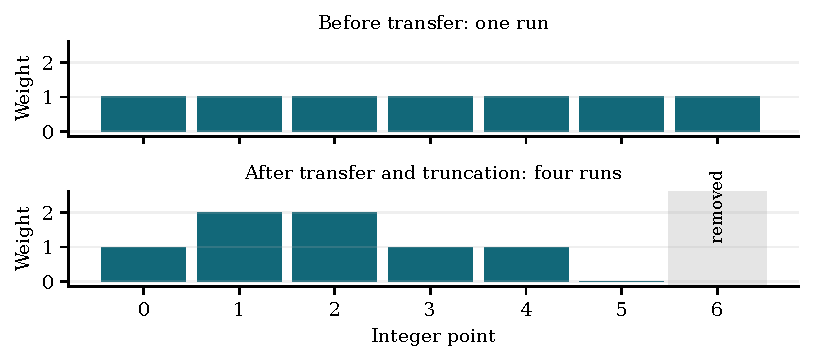
\includegraphics[width=0.84\textwidth]{sharp_transfer.pdf}
\caption{The exact seven-point example in the proof. Transferring the carrier
range $[5,7)$ to $[1,3)$ and removing point $6$ increases the number of
constant runs from one to four. Zero weight at surviving point $5$ remains
part of the representation.}
\label{fig:sharp-transfer}
\end{figure}

Static contraction cannot increase the number of weight runs: it merely
takes an ordered subsequence of point values and coalesces equal adjacent
runs. All other operations leave weights fixed. Consequently, after $T$
full transfers the current weight partition has at most $m_0+3T$ runs.
This bound is independent of the magnitudes of all represented intervals
and multiplicities. It remains valid with the Fine--Wilf merger because
that merger does not alter point weights or the equivalence relation.

For signed input weights let
$A=\sum_j (h_j-l_j)\|v_j\|_1$, using the additive input intervals.
Every intermediate coordinate has absolute value at most $A$: weights
are gathered, never copied into two different orbit representatives.
The bit length is therefore $O(1+\log(A+1))$, bounded by
$O(\log(N+1)+\log(m+1)+L+\log(d+1))$ when input coordinate bit length
is at most $L$. The degree-zero case is treated separately with empty
vectors. With the existing polynomial-size orbit trace, these facts give
polynomial bit complexity for canonicalization, all vector arithmetic,
and the compressed output. No new polynomial degree for the scheduler is
asserted. A simple bound on the number of emitted distinct records is the
number of trace contractions times $m_0+3T$, still polynomial.

\subsection{Sparse marked-component incidence}

For each of $r$ ports $A_i$ represented as a union of intervals, assign
coordinate $i$ of $w(x)$ to be $1$ if $x\in A_i$ and $0$ otherwise.
Normalize the intervals within each port so overlaps do not accidentally
count a point twice. The weighted output gives
\[
        W_i(O)=|O\cap A_i|,
\]
which contains both exact point multiplicity and the incidence signature
$\{i:W_i(O)>0\}$. Merge output vectors having the same support to obtain
a sparse histogram of attained signatures. Empty support is retained.
With $M$ marked intervals, this computation has polynomial bit complexity
in $k,M,r,\log(N+1)$; there is no $2^r$ output requirement. If the caller
requests a dense array indexed by every subset of $[r]$, that conversion
still requires $\Omega(2^r)$ slots. This sparse interface is an application
of the classical weighted theorem, not a new general result about AHT.

Additive incidence does not determine attachment order. A single circle
with four distinctly labelled marked points in cyclic order $a,b,c,d$
has the same weight vector $(1,1,1,1)$ as one with order $a,c,b,d$.
These orders are inequivalent under rotation and reversal with the labels
fixed. Thus even exact multiplicities and supports cannot recover the
ordered boundary data needed by a general cutting or gluing procedure.
Such a procedure must retain an additional order and transport structure.

\subsection{Connected normal-coordinate extraction}

For each of the at most $7t$ normal-disc types choose one incident local
edge. Add the corresponding basis vector at precisely the edge points
met by that disc stack on that chosen local edge. A triangle at vertex
$v$ occupies the points nearest $v$. On an edge directed $a$ to $b$, an
incident quadrilateral stack occupies the interval after the $a$-triangle
stack and before the $b$-triangle stack. The actual global edge orientation
may reverse the interval; obtain it from the validated parity data.
Different local edges may represent one global edge, so these basis
contributions are additive and must not overwrite each other.

Each local normal disc contributes one basis unit exactly once. Therefore
the orbit weight is the complete normal-coordinate vector of that actual
connected component. Grouped multiplicities encode equal components.
Their coordinate sum with multiplicity recovers the supplied vector.
This construction works for one-sided components directly and needs no
common-divisor reduction. In particular, $2$ times a one-sided component
may describe a connected two-sided double instead of two components;
the orbit extraction, rather than linear multiplicity guessing, decides
which occurs. This is the classical AHT Corollary 17 construction made
executable over the maintained edge-arc encoding.

Once weighted extraction has proved connectedness, Euler characteristic
one and nonempty boundary suffice to identify a disc, as proved in
Lemma~\ref{lem:disk-shortcut}. The existing torus-boundary homology test
then decides whether its boundary is essential. No further boundary or
orientation orbit query is needed. Extracting such a vector from
a disconnected input is new functionality of this code base. It does not
provide surface search, diagram-to-exterior provenance, hierarchy
construction, or a quasi-polynomial complete recognition procedure.

\subsection{Exact scope of replay and limits}

The weight certificate binds the normalized weight function and dimension,
the source-bound unweighted trace, and the ordered exact output classes.
Replay invokes no orbit scheduler. The ordinary orbit checker is
independent of orbit search. The weight producer and weight checker share
the small transport arithmetic; its independent validation comes from
the expanded graph and direct pushforward tests. Calling the entire
weight verifier arithmetically independent of weight production would
overstate this boundary.

The producer's cycle limit applies only to ordinary orbit search. The
weight-run, output-record and event limits are checked in the subsequent
weighted replay; the full ordinary trace has already been generated and
validated by then. They are cooperative work/output limits, not memory
or wall-clock guarantees. The standalone replay and weight-certificate
checker reject an over-limit trace by its explicit operation count before
ordinary proof replay. Every incomplete producer or standalone replay
returns no orbit count, class list, aggregate or certificate. Cancellation
exceptions propagate.


\section{From component vectors to an exact disk witness}
\label{sec:disk-extraction}

\subsection{A bounded-size anchor construction}

The arc encoding uses one point for each intersection of the surface with
a global triangulation edge. Normal arcs in faces pair appropriate
intervals of those points. Around a local normal disk the boundary arcs
connect all its corners, and gluing across faces identifies the same
surface. Consequently the connected components of this interval graph
are exactly the connected components of the normal surface.

For every active local disk type, choose one incident local edge and put
its coordinate basis weight at the corresponding stack of edge points.
Each disk contributes exactly once. The implementation explicitly maps
the chosen edge interval into the canonical global edge orientation;
identified local edges add weights at the same global points. The weight
dimension is $7t$, and the number of additive anchor intervals is at most
\[
        h\le 4t+q\le5t.
\]
Canonicalizing their endpoints therefore gives at most $2h+1\le10t+1$
initial weight runs. The face-arc construction uses at most $12t$
pairings, while $N\le4D$. The resulting weighted input is polynomial in
$t$ and $\log(D+1)$.

The output vector of an orbit has a stronger meaning than a compatible
summand of the input vector: it is the vector of one actual connected
component. This distinction matters because normal coordinate addition
can involve exchanges and reconnect summands. Verifying only that proposed
vectors are nonnegative, satisfy matching, and sum to the source would
not certify a component decomposition. The orbit trace supplies the
missing connectivity information.

The adapter revalidates each extracted vector against the finite geometry
and computes its Euler characteristic and boundary normal-arc count. It
also checks the exact conservation identity
\[
             \sum_{j=1}^{H}\mu_j f_j=f,
\]
where $f$ is the supplied vector and $\mu_j$ are binary multiplicities.
This is an additional consistency check, not a replacement for weighted
connectivity replay.

\subsection{Euler characteristic without expanded disks}

Let $T$ and $Q$ be the sums of the triangle and quadrilateral coordinates
of an extracted component. Its number of normal disks is $T+Q$, and its
number of local normal-arc occurrences is $A=3T+4Q$. If $B$ is the number
of normal arcs on unglued boundary faces, its surface cell structure has
$(A+B)/2$ edges: interior arcs are counted twice in $A$, while boundary
arcs are counted once. Its vertices are the distinct intersections with
global edges, counted by $N_f$. Thus
\begin{equation}\label{eq:euler}
             \chi(f)=N_f-\frac{A+B}{2}+T+Q.
\end{equation}
Every quantity is obtained by linear arithmetic on binary counts. No loop
over disks, arcs, or vertices is needed. The manifold and matching checks
ensure that these are the cells of the embedded surface being described.

\begin{lemma}[Connected disk shortcut]\label{lem:disk-shortcut}
Let $F$ be a connected compact surface. If $\chi(F)=1$ and
$\partial F\ne\varnothing$, then $F$ is a disk.
\end{lemma}
\begin{proof}
For an orientable connected surface with genus $g$ and $b\ge1$ boundary
components, $\chi=2-2g-b$. Equality to one forces $g=0$ and $b=1$.
For a nonorientable connected surface with $h\ge1$ crosscaps and
$b\ge1$, $\chi=2-h-b\le0$, so equality to one is impossible.
\end{proof}

The weighted orbit result already certifies connectedness. Consequently
the test $\chi(f_j)=1$ and $B_j>0$ suffices to recognize a disk component;
there is no need to run an orientation-double orbit computation or count
its boundary components separately. A closed projective plane has Euler
characteristic one but fails the boundary test, exactly as required.
This is a computational shortcut derived from information already proved,
not a change to surface classification.

\subsection{Essentiality on a torus must be tested per component}

A disk in a manifold is a compressing disk for its boundary if its boundary
curve is essential in that boundary. On a torus an embedded simple closed
curve is essential exactly when its mod-two homology class is nonzero.
Indeed, an essential curve has a primitive integral slope $(p,q)$; the
coordinates cannot both be even. Conversely, a contractible curve is
homologically zero. This uses the fact that the curve is a single embedded
simple closed curve, which the disk shortcut has established.

The existing finite boundary parity module constructs and independently
checks the corresponding cohomology witness. The new adapter invokes
that module only on extracted disk profiles. It never substitutes an
aggregate boundary class for the class of an individual disk. Two parallel
meridians have zero total class modulo two, although each bounds a
compressing disk. Such cancellation is one reason why component extraction
adds information that aggregate topology cannot provide.

For a boundary component of higher genus, an essential separating curve
may be homologically zero. The torus test would then be insufficient.
Extending the inventory to such manifolds is plausible, but extending its
essentiality conclusion requires a new boundary-curve decision procedure.
The current validator's torus hypothesis is part of the theorem used by
the implementation.

\subsection{A mixed surface with enormous multiplicities}

Take an eight-tetrahedron layered solid torus, a normal meridian disk with
vector $d$, and its boundary vertex-link disk with vector $\ell$. For
$K=2^b$, supply
\begin{equation}\label{eq:capacity-surface}
                 f=K d+(K+1)\ell.
\end{equation}
The vertex link can be taken in a sufficiently small vertex neighbourhood,
disjoint from the meridian. The components are $K$ meridian disks and
$K+1$ vertex-link disks. Their multiplicities are coprime. A global
greatest-common-divisor extraction cannot explain this decomposition.

The inventory returns two profiles, with total component count $2K+1$,
and identifies exactly $K$ compressing disks. The benchmark includes
$b=128,1024,4096,16384$; the final case represents
$2^{16385}+1$ connected components. It completes by transporting binary
weights on the same small combinatorial orbit trace. The certificate is
not constant size: its repeated endpoints and multiplicities must still
carry $O(b)$ bits. The complete serialized certificates and their sizes
are included in the results.

One-sided surfaces give a different reason to avoid multiplicity guessing.
A normal Möbius band with vector $m$ has a connected annular frontier with
vector $2m$. An odd multiple can contain both a Möbius component and
annular components. The extraction follows actual connectivity, so it
handles this directly. The next section proves that the number of distinct
profiles nevertheless remains linearly bounded by the triangulation and
the active quadrilateral support.

\section{A linear bound on distinct normal component vectors}
\label{sec:component-profile-bound}

Weighted orbit extraction produces a compressed inventory even when the
number of connected components is enormous. For an actual embedded normal
surface, its fully coalesced inventory satisfies a stronger, linear bound.
We prove it from normal-coordinate uniqueness and elementary normal
neighborhoods. This is a finiteness refinement for the present analysis;
we make no claim of literature-wide priority. Classical normal-surface
finiteness is discussed by King~\cite[Theorem 2]{king2003}, who attributes
the underlying result to Haken and Kneser and notes that stronger bounds
were already known.

Let $\mathcal T$ be a finite triangulation of a compact $3$-manifold $M$,
possibly with boundary. Tetrahedral faces may be identified within or
between tetrahedra, but the quotient must be a manifold: every vertex
link is a connected sphere or disc. Ideal vertices, singular vertex links,
and immersed surfaces are outside this statement. Write $t$ for the
number of tetrahedra and $v$ for the number of quotient vertices.
Orientability of $M$ is not required.

For a properly embedded normal surface $F$, its standard vector
$\mathbf x(F)\in\mathbb Z_{\ge0}^{7t}$ records four triangle counts and
three quadrilateral counts in each tetrahedron. These counts satisfy the
standard matching equations and the quadrilateral constraints. Standard
vectors determine normal surfaces up to ambient normal isotopy, including
their connected component multisets~\cite[Lemma 2.5 and Theorem 2.10]{burton2009}.
Let $Q(F)$ be the set of nonzero quadrilateral coordinates and put
$q=|Q(F)|\le t$. Count a component vector only once, regardless of how
many components have that vector, and denote the resulting number by $H$.

\begin{proposition}[Component-type bound]
\label{prop:component-type-bound}
Under these hypotheses,
\[
                     H\le v+2q.
\]
If every component of $F$ is two-sided, then $H\le v+q$.
Neither conclusion assumes incompressibility, least weight, or
fundamentality of $F$.
\end{proposition}

\begin{lemma}[Independence of disjoint two-sided types]
\label{lem:disjoint-normal-independence}
Mutually disjoint, connected, two-sided normal surfaces with pairwise
distinct standard vectors have linearly independent standard vectors.
\end{lemma}

\begin{proof}
Write the vectors as $\mathbf y_1,\ldots,\mathbf y_h$. Since their entries
are integers, a nontrivial real linear dependence implies a nontrivial
rational dependence: row reduction of the corresponding integer matrix
computes its kernel over $\mathbb Q$. Clearing denominators gives an
integer dependence. The vectors are nonzero and coordinatewise
nonnegative, so the nonzero coefficients cannot all have the same sign.
Consequently a dependence would give
\[
 \sum_{i\in P}a_i\mathbf y_i
       =\sum_{j\in R}b_j\mathbf y_j,
 \qquad a_i,b_j\in\mathbb Z_{>0},\quad P\cap R=\varnothing,
\]
with both index sets nonempty.

Choose mutually disjoint, sufficiently small normal product neighborhoods
of the surfaces. Two-sidedness permits any positive number of parallel
normal copies inside each such neighborhood, each with the same standard
vector as the original. The two sums therefore represent actual disjoint
unions having precisely the displayed component multisets. Equality of
their full vectors gives a normal isotopy between the unions. Such an
isotopy sends each connected component to a connected component and
preserves its normal-disc counts. Thus some $\mathbf y_i$ on the left
equals a $\mathbf y_j$ on the right, contradicting distinctness.
\end{proof}

\begin{proof}[Proof of Proposition~\ref{prop:component-type-bound}]
Let $V_Q\subseteq\mathbb R^{7t}$ be the real solution space of the
standard matching equations with all quadrilateral coordinates outside
$Q(F)$ set to zero. Project $V_Q$ to its $q$ permitted quadrilateral
coordinates. Its kernel has dimension exactly $v$.

Indeed, when every quadrilateral coordinate vanishes, face matching
identifies the triangle coefficients at the corners joined through that
face. The corner triangles around each quotient vertex have connected
adjacency graph, because its link is a connected surface. Their
coefficients must therefore agree. Values at different quotient vertices
are independent. The resulting basis consists of the vertex-link vectors
$\boldsymbol\ell_1,\ldots,\boldsymbol\ell_v$, each with one triangle at
every corner of its vertex and no other discs. Rank--nullity gives
\begin{equation}\label{eq:normal-support-dimension}
                  \dim V_Q\le v+q.
\end{equation}
In particular, every connected triangle-only normal surface is one
vertex link.

Choose one representative of each component type of $F$ having a nonzero
quadrilateral coordinate. Retain a two-sided representative unchanged.
Replace a one-sided representative $S$ by the horizontal frontier of a
small normal interval neighborhood. The frontier is the connected double
cover associated to the nontrivial normal line bundle of $S$; it is
two-sided and has standard vector $2\mathbf x(S)$. For a surface with
boundary, the vertical boundary of its interval neighborhood lies in
$\partial M$, and the horizontal frontier is properly embedded.

All these neighborhoods can be chosen mutually disjoint and disjoint
from retained representatives. Coalesce equal resulting vectors, and let
$r$ be their number. Adjoin all $v$ vertex links, taking them sufficiently
close to the triangulation vertices to avoid every chosen surface. The
resulting $r+v$ surfaces are mutually disjoint, connected and two-sided.
Their vectors are distinct: the first $r$ have nonzero quadrilateral
part, whereas vertex links do not. They lie in $V_Q$ and are independent
by Lemma~\ref{lem:disjoint-normal-independence}. Thus
\[
                r+v\le\dim V_Q\le v+q,
                \qquad r\le q.
\]

Each resulting nonvertex vector $\mathbf z$ has at most two original
preimages: a two-sided type with vector $\mathbf z$, and a one-sided
type with vector $\mathbf z/2$. Two different one-sided vectors cannot
have the same double. Hence there are at most $2r\le2q$ original
nonvertex types, and at most $v$ triangle-only types. This proves the
first bound. If all components are two-sided, the replacement map is
injective and the same argument gives $H\le v+q$.
\end{proof}

\subsection{A sharp one-tetrahedron example}

The factor two accounts for a real geometric possibility: a one-sided
component and its connected two-sided double can coexist. The fixture
\texttt{layered\_torus(1)} makes this explicit. Label the tetrahedron
vertices $0,1,2,3$, with face $i$ opposite vertex $i$, and identify face
$0$ with face $1$ by the permutation
$(0\,1\,2\,3)$; faces $2$ and $3$ remain boundary faces. This is a
one-vertex solid torus. Use coordinate order
\[
 (T_0,T_1,T_2,T_3;Q_{01|23},Q_{02|13},Q_{03|12}).
\]
Its vertex-link disc and a normal M\"obius band have vectors
\[
 \boldsymbol\ell=(1,1,1,1;0,0,0),\qquad
 \mathbf m=(0,0,0,0;0,1,0).
\]
For the single quadrilateral of $\mathbf m$, the corners on edges
$03,23,12$ become one vertex, while its corner on $01$ is another.
There are three edge cells and one face cell, so its Euler characteristic
is zero. The two unpaired sides form one boundary circle. The quotient
is therefore a M\"obius band. Its normal frontier is an annulus with
vector $2\mathbf m$.

Choose this band, its small frontier, and the vertex link disjointly.
Their union has vector
\[
 \boldsymbol\ell+3\mathbf m=(1,1,1,1;0,3,0)
\]
and exactly the three distinct component vectors
$\boldsymbol\ell,\mathbf m,2\mathbf m$. Thus $H=3=v+2q$ with $v=q=1$.
The union with vector $\boldsymbol\ell+2\mathbf m$ also attains the
two-sided bound $H=2=v+q$. The supplied native inventory and independent
Regina decomposition agree on these explicit components; the full fixture
and audit record are retained in
\texttt{results/normal\_inventory\_audit.json}.

\subsection{Consequences for encoded output}

Suppose the supplied coordinates have at most $B\ge1$ bits. Every
component coordinate is bounded by its source coordinate. A component
multiplicity is at most the total number of normal discs, hence needs
$O(B+\log(t+1))$ bits. Since $v\le4t$ and $q\le t$, the coalesced
normal inventory has
\[
             O\bigl(t^2(B+\log(t+1))\bigr)
\]
bits. The number of components itself remains unbounded for fixed
triangulation; it is their number of distinct full vectors that is linear.

AHT already establish polynomial-time recovery of component data from
binary normal coordinates~\cite[Corollary 17]{aht2006}. The present bound
sharpens the final output accounting and permits any polynomial-time
predicate on one connected vector to be evaluated on every type.
It does not enumerate candidate source surfaces. Nor does equality of
the weighted sum of proposed component vectors certify decomposition:
normal sums can reconnect surfaces, so actual component membership still
comes from the checked orbit calculation.

\section{Polynomial representation of raw singleton blocks}
\label{sec:persistent-elimination}

The existing word arena reconstructs substituted concatenations after every
acyclic elimination batch. Its one-batch polynomial bound does not, by
itself, give a polynomial bound for an arbitrary number of batches. We now
give a different representation with a bound for an entire sequence of raw
singleton eliminations. The representation has a tested reference
implementation, but it is not integrated into the knot-group producer or
the independent source-replay checker.

SLPs and their use in group presentations are established: for example,
Theorem 4.10 of Ennes and Maria's \emph{Compressed data structures for
Heegaard splittings} (arXiv:2507.11406v2) converts compressed relators to
a short ordinary presentation by introducing SLP nonterminals as Tietze
generators~\cite{ennesmaria2025}. The contribution here is an explicit representation, size
recurrence and prototype for the cumulative cost of a complete raw
singleton-elimination block. No claim of literature-wide priority is
needed for this refinement.

\subsection{Signed circuits and mutable generator bindings}

Fix a finite generator alphabet $X$ of size $r_0$. A signed handle $v$
references a circuit vertex; $-v$ represents the formal inverse word of
$v$. Vertex zero represents the empty word. There is one terminal vertex
for each positive generator, and immutable concatenation vertices
$c(u,v)$. Consequently
\[
 \operatorname{val}(-c(u,v))
 =\operatorname{val}(-v)\operatorname{val}(-u).
\]
Inversion requires no additional circuit vertices. Initially the circuit
is a binary SLP. Later, a terminal for an eliminated generator receives
one binding to a signed handle. An unbound terminal denotes its live
generator, while a bound terminal denotes the current value of its target.
All dependencies, including bindings, must form a directed acyclic graph.
Concatenation vertices retain their original children for the whole block;
only previously unbound generator terminals can acquire bindings.

The represented words are raw words. In particular, the adjacent letters
$x x^{-1}$ contribute two occurrences of $x$, even though their product
is trivial in the free group. This restriction makes a zero occurrence
count equivalent to the absence of a path to the corresponding live
terminal. It is essential to the proof below.

The current presentation retains the original list of relator slots.
Eliminating a generator clears exactly its chosen donor slot. Every other
root remains a reference to its existing circuit, so a new generator
binding applies the substitution to all retained relators simultaneously.
Historical donor vertices can remain allocated. Their continued presence
does not affect the presentation and is included in all size bounds.

\subsection{Position-free extraction of a singleton context}

Let $x$ be live and let a donor root represent
\[
   W=Lx^\varepsilon R,\qquad \varepsilon\in\{1,-1\},
\]
with exactly one occurrence of $x$ or $x^{-1}$. For this one generator,
compute counts in the three-element set $\{0,1,2\}$, where $2$ means
at least two. Counts add with saturation at concatenations, pass through
bindings, and are unchanged by orientation. A topological pass therefore
recognizes the singleton condition exactly. Counts need no expanded-length
integers, substring coordinates or word-equality oracle.

Starting at the donor root, follow its unique path to the live terminal
$x$. At a negative concatenation, reverse the order of the children and
negate their handles. At a binding, follow the bound handle with the
appropriate sign. At each concatenation on the path, exactly one child
contains $x$ and the other contains none. Save this other child as a
signed sibling handle. Siblings before the path form $L$ in descent order;
siblings after the path form $R$ in reverse descent order. This yields an
ordered list of existing signed handles for $RL$.

Combine the list by balanced pairwise concatenation. If there are $q$
nonzero handles, at most $\max(0,q-1)$ new concatenation vertices are
needed, and every path through the new concatenations has length at most
$\lceil\log_2\max(1,q)\rceil$. The balancing is by the number of sibling
handles, not by the expanded lengths of their values. Interning repeated
concatenations is optional and can only reduce allocation.

Install the binding
\begin{equation}\label{eq:persistent-binding}
 x\longmapsto
 \begin{cases}
   (RL)^{-1},&\varepsilon=1,\\
   RL,&\varepsilon=-1.
 \end{cases}
\end{equation}
This is the familiar exact solution of $Lx^\varepsilon R=1$.

\paragraph{Lemma (acyclicity and simultaneous substitution).}
The binding in \eqref{eq:persistent-binding} preserves acyclicity and
applies exactly the corresponding singleton Tietze elimination to all
retained roots.

\begin{proof}
Before the binding is installed, every saved sibling has occurrence count
zero for $x$. Hence its old dependency graph has no path to the live
terminal $x$. The new image consists only of these siblings and new
concatenations. It consequently has no path to $x$. Any newly created
directed cycle would have to use the new edge out of $x$ and then return
from the image to $x$, which is impossible.

Let $\phi$ evaluate the old binding graph as raw words in the live
alphabet, and let $\sigma$ replace $x$ by the raw word specified in
\eqref{eq:persistent-binding}. Evaluation of the enlarged acyclic graph
is $\sigma\circ\phi$: this follows directly by induction over its
dependency order, with the only changed terminal being $x$. In
particular, bindings of earlier eliminated generators update their values
automatically. Deleting the donor equation and eliminating $x$ is an
elementary Tietze transformation, so the presented group is preserved.
\end{proof}

The no-path argument remains valid even when a later image references an
earlier eliminated terminal. If that earlier terminal could lead back to
the current generator, its occurrence count in the proposed image would
be positive and it could not be a saved sibling. No fixed elimination
order on original generator labels is required.

\subsection{The global size theorem}

Write $S_0$ for the initial number of nonzero vertices and $D_0$ for the
largest number of concatenation vertices on a dependency path in the
initial SLP. Suppose that exactly $k\le r_0$ distinct live generators are
eliminated, with no intervening free reductions, new generators, or other
word transformations. Donors may be chosen adaptively, but each must
satisfy the raw singleton condition at the time it is used.

After $i$ eliminations let $D_i$ be the largest number of concatenation
vertices on a path when all generator bindings are ignored, and let
$H_i$ be the longest full dependency path, counting concatenations and
binding edges. At most $i$ bindings lie on any full path: a directed
acyclic path cannot visit a terminal twice. Such a path splits into at
most $i+1$ binding-free segments. Therefore
\begin{equation}\label{eq:persistent-height}
 H_i\le(i+1)D_i+i < (i+1)(D_i+1)=:A_i.
\end{equation}
The singleton descent encounters at most $H_i$ concatenations, so its
sibling count $q_i$ is at most $A_i$. Balanced construction gives the
recurrence
\begin{equation}\label{eq:persistent-recurrence}
 D_{i+1}\le D_i+
       \left\lceil\log_2\max(2,A_i)\right\rceil.
\end{equation}

\paragraph{Theorem (complete raw singleton blocks have polynomial size).}
For every $0\le i\le k$,
\begin{equation}\label{eq:persistent-D}
 D_i\le D_0+6i\log_2(D_0+i+2).
\end{equation}
In particular, putting $T=D_0+k+2$, the number $S_k$ of allocated
nonzero vertices satisfies the explicit bound
\begin{align}\label{eq:persistent-S}
 S_k\le S_*:={}&S_0+\frac{k(k+1)}2(D_0+1)\notag\\
 &\quad+2k(k-1)(k+1)\log_2 T.
\end{align}
The bit length $B_k$ of every represented raw length, including historical
roots and image vertices, satisfies
\begin{equation}\label{eq:persistent-B}
 B_k\le(k+1)\bigl(D_0+6k\log_2 T+1\bigr).
\end{equation}
Thus
\[
 S_k=O\bigl(S_0+k^2(D_0+1)+k^3\log(D_0+k+2)\bigr),
\]
and a whole block has polynomial encoded complexity in the initial
grammar size and rank, even if it uses a linear number of serial phases.

\begin{proof}
Set $T_i=D_0+i+2\ge2$. The claim for $D_0$ is immediate. Suppose that
\eqref{eq:persistent-D} holds at $i$. Since $i+1\le T_i$,
$D_0+1\le T_i$, and $i\le T_i$, we obtain
\[
 A_i\le T_i^2(1+6\log_2 T_i)\le T_i^5.
\]
For the final inequality it suffices to observe that
$\log_2 t\le t-1$ for $t\ge2$, and
$6t-5\le t^3$ on the same range. The latter follows because
$t^3-6t+5$ is positive at $t=2$ and has positive derivative thereafter.
As $T_i^5\ge2$, it follows that
\[
 \left\lceil\log_2\max(2,A_i)\right\rceil
 \le5\log_2 T_i+1\le6\log_2 T_i.
\]
Substitution into \eqref{eq:persistent-recurrence} yields
\[
 D_{i+1}\le D_0+6(i+1)\log_2 T_i
          \le D_0+6(i+1)\log_2 T_{i+1},
\]
completing the induction with the stated constant.

At step $i$, no generator vertex is added and at most $q_i\le A_i$
concatenation vertices are allocated. Sum
\[
 A_i\le(i+1)(D_0+1)+6i(i+1)\log_2 T
\]
over $i=0,\ldots,k-1$. The identities
\[
 \sum_{i=0}^{k-1}(i+1)=\frac{k(k+1)}2,\qquad
 \sum_{i=0}^{k-1}i(i+1)=\frac{k(k-1)(k+1)}3
\]
give \eqref{eq:persistent-S}.

Unfolding a binary/unary acyclic circuit of height $H_i$ gives a tree
with at most $2^{H_i}$ terminal leaves. Inversion does not change length,
and bindings are unary. Hence every represented length has bit length
at most $H_i+1$. Combine this observation with
\eqref{eq:persistent-height} and \eqref{eq:persistent-D} to obtain
\eqref{eq:persistent-B}. Empty values have bit length zero and satisfy
the same bound.
\end{proof}

\subsection{Running time and ordinary SLP export}

For a supplied sequence of donor slots and live generator labels, the
reference algorithm performs a topological pass and a capped occurrence
pass over all historical vertices at each step. The graph has at most
two outgoing edges per vertex. Context extraction and balanced assembly
take $O(q_i)$ further operations. The whole block therefore uses
$O(kS_*)$ graph operations beyond initial input handling. If $M$ is the
original number of relator slots, reading the input and exporting its roots
add $O(S_0+M)$ operations; the total, including final export, is
$O(S_0+M+kS_*)$. Working storage is $O(S_*+M)$, including the fixed
relator-root list and the $k$ binding entries. The exported root list uses
$O(M\log(S_*+r_0+2))$ bits. Input labels may be
renumbered densely once; node identifiers use
$O(\log(S_*+r_0+2))$ bits.

This count requires neither large-integer lengths nor exact string
equality. A deterministic implementation can omit interning and use dense
arrays for all generator and vertex metadata. If interning is desired,
balanced comparison dictionaries give a conservative
$O(kS_*\log^2(S_*+r_0+2))$ bit-operation accounting in the usual
bit-cost random-access model. The Python prototype uses hash dictionaries;
its measured timings do not constitute that deterministic machine bound.

Adaptive donor discovery remains polynomial within this raw-only model:
one may compute the same saturated counts for each live generator and
scan every retained root, adding a factor at most $r_0$ to the graph
passes plus the root-scanning cost. This observation gives no guarantee
that another singleton donor exists, that a chosen order reaches rank
one, or that searching over many alternative orders is cheap.

The representation is not a permanent barrier to existing word kernels.
At an explicit end-of-block boundary, topologically evaluate each vertex
in both orientations. A bound generator becomes an alias to its image;
an unbound generator becomes its positive and negative terminal letters;
a concatenation becomes two ordinary concatenations with opposite child
orders and signs. This exports a standard binary SLP containing at most
$2S_k$ nonzero vertices, with all references in allocation order and no
bindings. The export is linear in circuit size. It is implemented by
\texttt{export\_slp} in the prototype and checked against a separate
literal reconstruction on the finite tests.

A single existing polynomial compressed free-reduction operation
\cite{schleimer2008} can
therefore be charged after the export. The theorem does not cover a
repeated alternation of normalizations and other presentation moves.
Nor does it automatically include torsion-dependent primitive-power
quotients whose donor generator is not a raw singleton. Those operations
require their own growth analysis.

\subsection{A controlled family with exponentially long raw contexts}

Let the generators be $a,b,x_0,\ldots,x_k,z$, and take
\[
 r_0=x_0^{-1}a x_1 b,\qquad
 r_i=x_0^{-1}x_{i+1}\ (1\le i<k),\qquad
 r_k=x_0^{-1}z.
\]
Eliminate $x_i$ from the current value of $r_i$, successively for
$i=0,\ldots,k-1$, and retain $r_k$. After the first elimination,
$x_0=A_1x_1B_1$ with $A_1=a$, $B_1=b$. If after step $j$ it is
$A_jx_jB_j$, the next donor gives
$x_j=A_j^{-1}x_{j+1}B_j^{-1}$, so
\[
 A_{j+1}=A_jA_j^{-1},\qquad B_{j+1}=B_j^{-1}B_j.
\]
These are raw words, so $|A_j|=|B_j|=2^{j-1}$ and the retained relator
has length $2^k+2$. All selected pivots remain singletons. This artificial
presentation family stresses retained contexts and repeated substitutions;
it is not a family of difficult knot diagrams. Free reduction would
remove its deliberately retained cancellation padding.

The benchmark compares the new circuit with the pinned repository's
\texttt{apply\_batch} called with the very same one-entry donor sequence.
Both arms start from the same explicit source relators, clear the same
slots, retain raw words, and disable their expansion method. An identical
eager control measures scheduling variability. There is one excluded
warm-up per size and arm, followed by five randomized A/A/B rounds.
Timing includes source construction and all eliminations; final diagnostic
measurements are excluded. Both arms use caps of two million vertices
and one billion implementation work units, and every run completes.

\begin{center}
\begin{tabular}{r|rrr|rr}
 $k$ & Eager (s) & Control (s) & Persistent (s)
     & Eager vertices & Persistent vertices\\\hline
 8   & 0.000879 & 0.000869 & 0.000363 & 238 & 83\\
 16  & 0.005813 & 0.005988 & 0.001871 & 914 & 279\\
 32  & 0.043468 & 0.045512 & 0.010994 & 3610 & 839\\
 64  & 0.341194 & 0.348591 & 0.067422 & 14378 & 2534\\
 128 & 2.853190 & 3.013364 & 0.395421 & 57418 & 6890
\end{tabular}
\end{center}
The final row gives a measured median speedup of about $7.22$ relative
to the eager arm. Its retained word has length $2^{128}+2$. The new
representation has 128 extra binding entries in addition to its 6,890
vertices, and uses signed handles instead of separate inverse subgraphs;
vertex counts are consequently structural counts, not byte measurements.
Both sides retain historical vertices. Work counters have different
charging conventions and should not be interpreted as portable CPU
instruction counts.

The six test methods include 600 deterministic random presentation traces
checked against independently implemented literal substitution, explicit
negative handles and empty images, repeated-child rejection, forward
bindings, interruption before a binding is published, and the 128-step
capacity example with expansion disabled. The tests check the syntactic
height recurrence and the $2S_k$ export bound as well. These are tests of
word representation and Tietze semantics; no new knot verdict is produced.

\subsection{Consequences and next questions}

The size theorem removes a logarithmic-phase hypothesis from this
restricted raw singleton-elimination component, provided the persistent
representation is used. It does not establish a quasi-polynomial
unknot-recognition algorithm. The implementation work needed before
production use is concrete: add a source-derived replay path; preserve
all presentation-slot and cancellation semantics; implement a compatible
raw donor planner; export exactly at normalization boundaries; and measure
complete discovery and replay on real diagrams. Algebraically, the next
questions are whether the cubic logarithmic size term can be improved,
whether suitable normalization steps preserve a comparable amortized
bound, and which topologically meaningful diagram classes admit enough
raw singleton eliminations to reach a checked terminal presentation.


\section{Implementation, independent checks, and measurements}
\label{sec:experiments}

\subsection{What changed in the maintained code}

The integration patch adds three production-capable geometry modules and
three test modules. It does not alter existing recognition dispatch or
replace the dense incidence API. The additions are
\code{weighted\_orbits.py}, \code{sparse\_port\_incidence.py}, and
\code{normal\_components.py}. The persistent circuit remains an explicitly
separate research prototype in the experiments directory, pending the
planner and source-replay work described below.

The supplied patch applies to the pinned commit; the accompanying source
snapshot includes the unchanged dependencies needed for independent
reproduction. Historical tests import small reference implementations from
four sibling report directories. Those fixtures and their original licences
are included with their hashes. The first attempt to run the full suite
failed at import/setup because those sibling files were absent from the
sparse checkout. Restoring the unchanged pinned fixtures resolved that
environment problem; the original failed log is retained rather than
silently discarded.

\subsection{Tests that exercise mathematical failure modes}

The final maintained suite reports \FullTests{} passing test methods, with
Regina available. Of these, 26 are the new geometry methods: 14 for weighted
orbits, five for sparse incidence, and seven for component extraction.
The separate persistent-circuit suite has six passing methods. These
method counts understate the number of mathematical instances, because
the methods contain deterministic exhaustive and randomized comparisons.

\begin{table}[htbp]
\centering\small
\begin{tabularx}{\textwidth}{@{}p{0.29\textwidth}rY@{}}
\toprule
Audit & Instances & Independent comparison or property\\
\midrule
Small weighted orbit systems & 15,816 & Expanded union-find orbit sums for all
systems with at most two pairings and binary point weights through universe size four\\
Signed vector weights & 2,500 & Expanded signed three-coordinate orbit sums;
150 also checked with the classical merger\\
Full-range transfers & 5,000 & Literal pointwise pushforward versus compressed folding\\
Sparse incidence & 250 & Existing dense histogram versus sparse attained supports\\
Focused normal extraction & 72 & Exact Regina component-coordinate multisets\\
Broader normal audit & 1,000 & Regina components, topology, disk status,
source-bound replay, and profile inequalities\\
Persistent elimination & 600 traces & Separate literal substitution oracle;
more than 1,000 successful eliminations\\
\bottomrule
\end{tabularx}
\caption{Mathematical comparison workloads, in addition to malformed-input,
resource, cancellation, and source-binding tests. Instance collections may
overlap and are not added to obtain a misleading single total.}
\label{tab:audits}
\end{table}

The weighted tests include zero-dimensional vectors, negative weights,
the sharp three-run example, and analytic systems with 18,001-bit
endpoints. They mutate weights, dimensions, multiplicities, source pairings,
and local proof records. Verification is also exercised with the orbit
search function replaced by a function that raises if called. Certificate
schema validation rejects Boolean values masquerading as integers.

The broader normal audit uses eleven finite triangulations, including
layered solid tori, boundary-cap extensions, an interior vertex subdivision, and a solid
torus connected-summed with $\mathbb{RP}^3$. The last fixture deliberately
tests geometry beyond knot exteriors. It includes 200 relabelings and 63
random compatible sums, with 150 cases containing nonorientable boundary
surfaces and 26 containing closed nonorientable surfaces. There are 116
cases with compressing disks. All 1,000 component multisets agree exactly
with Regina. The stronger two-sided profile bound is checked in all 824
applicable cases. Every certificate replays with both orbit and parity
search disabled. These are independent finite checks, not substitutes for
the proofs.

\subsection{Geometry timing protocol}

Measurements use Python 3.12.14 on the recorded Linux x86-64 environment,
with Regina engine 7.4 and distribution 7.4.1 for the independent audits.
Comparative timings run without concurrent audit or full-suite workloads.
Before and after each experiment the scripts hash the relevant source
files and require equality. All raw samples, shuffled orders, exact inputs,
completion statuses, and structural counters are retained.

The primary geometry experiment has thirteen cases and four arms:
the existing dense query, an identical dense control, the new sparse
query, and the new query followed by certificate verification. Each case
has one excluded warm-up per arm and five measured shuffled rounds,
giving 260 measured calls. Timing covers the complete call. Histogram
comparison is outside the timing interval; proof replay is inside the
verified arm. No local resource cap censors these runs.

The cases distinguish disjoint, nested, and coincident ports. Static
systems on $2^{512}$ points expose the unavoidable cost of dense output
without geometric scheduling work. Native interval systems come from
an eight-tetrahedron normal meridian and from $2^{64}$ parallel meridians.
These are supplied normal surfaces, not knot-recognition benchmarks.

\begin{table}[htbp]
\centering\small
\setlength{\tabcolsep}{4pt}
\begin{tabular}{@{}lrrrrr@{}}
\toprule
Case & Dense & Sparse & Sparse + replay & D/S & A/A\\
\midrule
Static, disjoint, $r=4$ & 0.451 & 0.126 & 0.201 & 3.06 & 1.05\\
Static, disjoint, $r=8$ & 15.045 & 0.184 & 0.324 & 81.55 & 0.97\\
Static, disjoint, $r=12$ & 477.954 & 0.323 & 0.685 & 1390.69 & 1.05\\
Static, nested, $r=12$ & 15.368 & 0.241 & 0.496 & 61.42 & 0.98\\
Static, identical, $r=12$ & 15.384 & 0.158 & 0.343 & 99.07 & 0.99\\
Meridian, disjoint, $r=4$ & 12.606 & 2.496 & 3.604 & 5.04 & 1.05\\
Meridian, disjoint, $r=6$ & 38.299 & 2.908 & 4.212 & 14.07 & 0.99\\
Meridian, disjoint, $r=8$ & 171.075 & 3.063 & 4.735 & 56.36 & 0.99\\
Meridian, identical, $r=8$ & 3.223 & 2.522 & 3.348 & 1.23 & 0.98\\
Parallel, disjoint, $r=4$ & 25.029 & 2.913 & 4.364 & 8.66 & 1.00\\
Parallel, disjoint, $r=6$ & 94.974 & 3.269 & 4.868 & 28.99 & 1.00\\
Parallel, disjoint, $r=8$ & 382.624 & 3.612 & 5.937 & 107.92 & 1.00\\
Parallel, identical, $r=8$ & 6.542 & 2.721 & 3.584 & 2.29 & 1.01\\
\bottomrule
\end{tabular}
\caption{Final primary geometry experiment. Times are median milliseconds per complete call. D/S and A/A are medians of paired dense/sparse and dense/control ratios. The full JSON retains all four arms and all samples.}
\label{tab:geometry}
\end{table}


The median paired ratio is formed inside each shuffled round and then
aggregated; it need not equal the ratio of the two displayed medians.
The A/A column is the dense median paired ratio against its identical
control. Values away from one expose the variability of these short
measurements. Large disjoint-port gains are consistent with eliminating
the dense subset enumeration. Small gains or reversals are treated more
cautiously, especially where identical ports already benefit from the
baseline's marked-union reuse.

\begin{figure}[htbp]
\centering
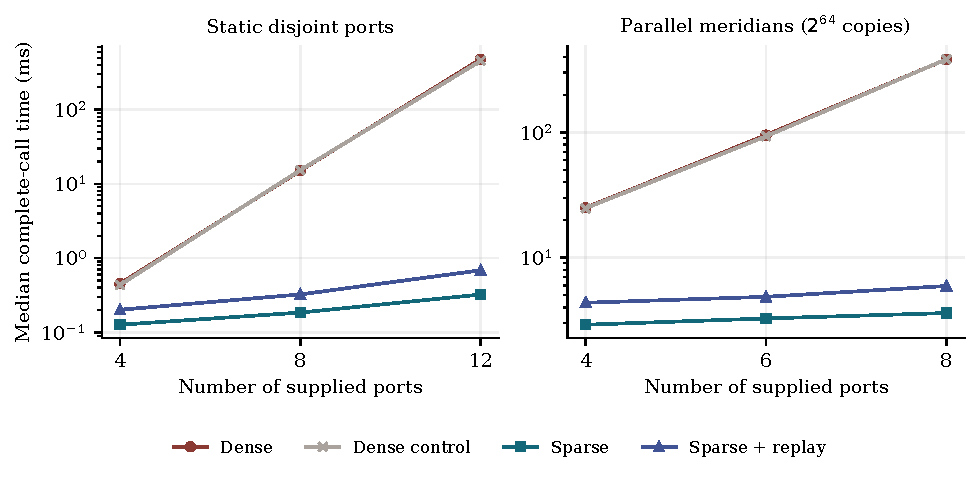
\includegraphics[width=\textwidth]{geometry_scaling.pdf}
\caption{Completed dense and sparse port queries on the final source.
The horizontal axis counts explicit ports. Static disjoint ports isolate
the dense output cost; the native parallel-meridian cases also exercise
the interval scheduler. The axes are logarithmic where indicated.
Points are medians, not fitted complexity exponents.}
\label{fig:geometry}
\end{figure}

\subsection{Batched follow-up and compressed capacity}

The initial measurement pass showed material A/A variation on small
queries. The final primary pass and a separate follow-up are both retained;
the original pass is labelled as a development snapshot because minor
cancellation-polling corrections followed it. The follow-up uses repeated
complete calls within each timed batch for four predetermined small or
noisy cases, with seven shuffled rounds. It reports time per call and
does not replace the primary experiment selectively.

\begin{table}[htbp]
\centering\footnotesize
\setlength{\tabcolsep}{4pt}
\begin{tabular}{@{}lrrrrrrr@{}}
\toprule
Case & Batch & Dense & Sparse & Verified & D/S & D/V & A/A\\
\midrule
Static, disjoint, $r=4$ & 128 & 0.324 & 0.049 & 0.117 & 6.474 & 2.715 & 0.995\\
Static, nested, $r=12$ & 8 & 14.763 & 0.179 & 0.427 & 81.711 & 33.724 & 0.988\\
Meridian, identical, $r=8$ & 16 & 2.811 & 2.087 & 2.974 & 1.404 & 0.945 & 1.007\\
Parallel, identical, $r=8$ & 16 & 5.793 & 2.481 & 3.544 & 2.324 & 1.621 & 1.002\\
\bottomrule
\end{tabular}
\caption{Batched follow-up: median milliseconds per call; seven paired rounds, 4,704 measured calls and 672 excluded warm-up calls. D/V compares dense counting with sparse counting plus proof replay. The 0.945 ratio is a retained regression.}
\label{tab:batched}
\end{table}


Capacity records are separate from comparative timing. They include
the mixed normal surfaces in \eqref{eq:capacity-surface} and static sparse
systems with 32, 128, and 512 disjoint ports. The latter return respectively
32, 128, and 512 attained signatures. There is no attempt to allocate a
dense $2^{512}$-entry output, and no claimed measured speedup against such
an uncompleted allocation.

\begin{table}[htbp]
\centering\small
\setlength{\tabcolsep}{4pt}
\begin{tabular}{@{}rrrr@{}}
\toprule
$b$ in $K=2^b$ & Produce + replay (ms) & Certificate bytes & Profiles\\
\midrule
128 & 49.24 & 37,072 & 2\\
1024 & 48.51 & 118,337 & 2\\
4096 & 54.20 & 334,975 & 2\\
16384 & 77.06 & 1,259,441 & 2\\
\bottomrule
\end{tabular}
\caption{Single completed capacity probes for $K d+(K+1)\ell$ in an eight-tetrahedron solid torus. These are individual capacity observations, not repeated timing estimates or comparative speedup claims.}
\label{tab:capacity}
\end{table}


For the eight-tetrahedron mixed surfaces, the weighted trace has the same
275 explicit events, 23 scheduler cycles, and 22 transfers across these
bit lengths. It uses 40 anchor intervals, dimension 56, and 35 initial
and peak weight runs. The benchmark demonstrates that enormous
multiplicities do not force enumeration. It also shows the real encoded
cost: the largest certificate contains \LargestCertificateBytes{} bytes
in the stated JSON format. Hexadecimal transport avoids changing Python's
process-wide decimal conversion limit. Compression of the distribution
archive is separate from the certificate's mathematical bit-size bound.

\subsection{What the word measurements establish}

The persistent-elimination section gives all five rows of the A/A/B
comparison and describes the exact artificial source family. At 128
eliminations the new prototype takes about 0.395 seconds versus 2.853
seconds for eager serial elimination, a ratio of median times of about
7.22. Both complete, use the same supplied donors, and keep expansion
disabled. The retained raw relator has length $2^{128}+2$.

This family was chosen to exercise repeated retained contexts. Its freely
cancelling padding means that it would be inappropriate to present it as
a difficult family for the full knot algorithm. The experiment supports
the practical value of this particular representation and the structural
bound; it does not establish an exponential lower bound on the old arena,
whose measured vertex growth on this family is quadratic. A future
integration benchmark must include donor discovery, normalization, source
replay, and actual knot diagrams.

\FloatBarrier
\section{Certificate contracts and integration design}
\label{sec:contracts}

\subsection{The weighted proof interface}

The weighted certificate contains a version, a dimension, the canonical
complete weight partition (including zero runs), ordered output classes, and the
source-bound ordinary orbit certificate. A class is serialized as
\code{[vector,multiplicity]}; it is not one object per connected component.
The verifier reconstructs the claimed weights from the explicit source
arguments, checks the ordinary orbit proof, and replays every weight
transfer and static emission, comparing the exact ordered classes with the
claim. The producer and standalone replay utility also check total orbit
multiplicity and the aggregate vector explicitly.

The ordinary orbit checker is independently implemented relative to the
scheduler. Weighted production and weighted verification share the small
transport arithmetic, as does normal geometry reconstruction. Their
independent validation is supplied by the expanded finite oracles and
the Regina component comparisons. This separation should remain visible
in documentation and future proof audits: invoking a shared function twice
does not create an independent arithmetic implementation.

The sparse certificate additionally binds the normalized input ports and
the attained histogram. The normal-component certificate binds the
triangulation and original vector, the weighted proof, the exact profiles,
and the independently checked boundary parity records. For a disk profile
the verifier derives its boundary graph from the source geometry and
the extracted coordinates. It does not trust a supplied assertion of
connectedness, Euler characteristic, or essentiality.

\subsection{Input provenance and the meaning of a negative result}

The normal inventory's mathematical statement is: these are the connected
components of this supplied normal surface in this supplied triangulation.
A compressing disk is therefore a witness about that manifold. Relating
it to an original knot diagram additionally requires a checked conversion
from the diagram to its exterior and checked transport through all
simplifications. The new modules do not silently inherit that provenance
from a filename, hash, or external-engine claim.

Similarly, an inventory with no compressing disk proves only that this
particular supplied surface has no such component. It does not prove
that the manifold has incompressible boundary. The empty vector gives
an empty inventory, not evidence of knottedness. A future complete
procedure needs a justified way to choose surfaces or certify a hierarchy.
The same logical distinction applies to the word prototype: exhausting
all raw singleton donors is an algebraic stopping condition, not a proof
that the knot is nontrivial.

\subsection{Resource and cancellation semantics}

The cycle allowance is charged by ordinary orbit discovery. The weighted
producer currently first builds and checks that ordinary trace, then
applies its weight-run, output-record, and event allowances during weighted
replay. Thus these limits do not bound the earlier trace allocation.
Standalone weighted replay and certificate verification can reject an
overlong explicit trace before running ordinary replay, but they still
receive an already materialized input object.

These are cooperative work and output allowances. They are not promises
about process memory, JSON parser allocation, or wall-clock latency.
Callbacks are polled in the source and certificate loops; callback
exceptions propagate instead of being mistaken for malformed data.
An incomplete weighted result has no count, class list, aggregate, or
certificate, and the higher-level adapters return an inconclusive status.
The implementation never presents a partial inventory as complete.

For the persistent circuit, a failed or interrupted construction may
allocate unreachable temporary concatenations before publishing a binding.
The mathematical size theorem counts a completed valid block from a fixed
initial circuit; repeated failed attempts that leave orphan allocations
are not free. A production transactional wrapper should roll back those
allocations, collect unreachable nodes, or include their costs explicitly
in the potential function. The current tests check that an interrupted
operation does not publish a false generator binding.

\subsection{A concrete integration sequence}

The geometry patch can be reviewed and applied without changing the
recognizer's existing decisions. Its first callers should be offline
normal-surface and boundary-pattern experiments. Such callers can reuse a
single inventory for disk selection and support queries. If they truly
need a dense table, an explicit final conversion preserves that interface
and acknowledges its output cost.

The persistent circuit needs more work before production use. Its mutable
generator bindings change the values of previously allocated nodes.
Existing caches in the immutable word arena cannot be reused unchanged.
Occurrence counts, lengths, Whitehead summaries, and donor frontiers need
a dependency-aware invalidation policy or an explicit recomputation phase.
The proposed first integration should keep a raw-only block, recompute
saturated donor counts, and export once at the normalization boundary.

For independent replay, each pivot image must be derived from the
source-bound donor and its unique raw occurrence. A certificate may specify
the donor slot and live generator, but it must not be allowed to supply an
unverified replacement image. The checker can independently reconstruct
the signed circuit and compare the final exported presentation with the
existing terminal certificate contract. Replacing a search arena alone
does not establish this proof path.

The final acceptance experiment should compare the complete integrated
pipeline with identical resource conventions, retain unchanged-case
controls, report every timeout as censored, and include native hard-knot
and hard-unknot families. That experiment is intentionally a future
milestone: the current package contains kernels and a representation
prototype, with their exact scope documented.

\section{Cost composition and the next research obligations}
\label{sec:research-agenda}

The results above improve two representation costs: extracting the
components of a supplied normal surface, and retaining a complete block
of raw singleton substitutions. The next theorem states precisely how
such local improvements could contribute to a complete recognition bound.
It also makes clear which quantities future work must control.

\subsection{A conditional theorem for the whole computation}

Let $n\ge2$ be the bit length of a diagram encoding. Standard encodings
whose size is polynomial in the crossing count give the same
quasi-polynomial complexity class. All subsequent sizes are measured in
bits, including integer coordinates, combinatorial incidence, word
circuits, retained history and proof references.

\begin{proposition}[Conditional cost composition]
\label{prop:conditional-cost-composition}
Suppose a deterministic algorithm constructs and evaluates a search tree
for an input of size $n$, subject to the following uniform bounds.
The transition and terminal rules are sound, and exhausting the tree is
complete for both unknot and knotted verdicts. The tree has depth at most
$h=h(n)$, and each node at depth $j<h$ has at most $b_j=b_j(n)\ge1$
children. Failed candidate attempts and repair iterations are included
in the tree or in its explicitly charged node work.

Every intermediate state has at most $s=s(n)\ge1$ bits. All work at
one node, including generation of its candidates and rejected proposals,
has bit cost polynomial in $n+s$, with one polynomial independent of the
input and node. Each node contributes at most polynomially many bits in
$n+s$ to a source-bound proof record. The assembled proof is independently
checkable in time polynomial in its full length and $n$.

Then there is an absolute constant $a$ such that discovery, proof output,
and independent verification together have cost at most
\begin{equation}\label{eq:global-composition-cost}
 \left((h+1)(n+s+2)\prod_{j=0}^{h-1}b_j\right)^a.
\end{equation}
In particular, for a fixed $c\ge1$, the sufficient condition
\begin{equation}\label{eq:global-log-budget}
 \log_2(n+s+2)+\log_2(h+1)
       +\sum_{j=0}^{h-1}\log_2 b_j
       =O\bigl((\log n)^c\bigr)
\end{equation}
gives a complete deterministic recognition algorithm of complexity
$2^{O((\log n)^c)}$.
\end{proposition}

\begin{proof}
The number of nodes at depth $j$ is at most
$\prod_{i=0}^{j-1}b_i$. Since every $b_i\ge1$, the total node count is
at most $V=(h+1)\prod_{i=0}^{h-1}b_i$. Summing the uniform node cost
and proof length gives $V(n+s+2)^{O(1)}$ for each. Applying the assumed
polynomial verifier to that full proof preserves a fixed polynomial in
$V$ and $n+s+2$, proving~\eqref{eq:global-composition-cost}. Taking
logarithms gives~\eqref{eq:global-log-budget}. Soundness and completeness,
which are separate hypotheses, turn this computation bound into a
recognition bound.
\end{proof}

For example, $s=n^{O(1)}$, $b_j=n^{O(1)}$ uniformly, and
$h=O(\log n)$ give $2^{O((\log n)^2)}$. Replacing the depth by
$O((\log n)^2)$ gives $2^{O((\log n)^3)}$. A deterministic chain with
polynomially many steps and polynomial state size needs no logarithmic-depth
hypothesis: its branching factors are all one. A small description of each
state does not establish the branching term; polynomial-time operations
do not establish a bound on the largest state. If the terminal rules
only certify unknottedness, the same analysis bounds a possibly
inconclusive positive search and does not supply the missing negative
verdict.

The analogous accounting for an iteration bound $L(g+1)^L$, as in
Lackenby's hierarchy analysis~\cite[Proposition 9.1]{lackenby2026}, is
\[
 \log_2(n+s+2)+\log_2(L+1)+L\log_2(g+1)
                  =O((\log n)^c).
\]
This is conditional on bounded candidate generation, repairs and replay
throughout the computation. Bounds for an essential boundary pattern
cannot simply be applied to arbitrary unsuccessful branches.

\subsection{Prioritized questions and concrete targets}

The following questions are ordered by their role in completing the
geometric and algebraic pipelines. Each asks for a specific constructive
result or obstruction, rather than an improvement to isolated timings.

\begin{enumerate}
\item \textbf{How can a useful surface be found?}
Can one generate a complete family of useful normal or hierarchy surfaces
after $2^{\operatorname{polylog} n}$ candidate attempts, with uniformly
bounded encoded coordinates? Component extraction now permits a candidate
to be disconnected. The missing statement concerns coverage: whenever
the required compression or hierarchy move exists, some generated
candidate must contain it. A first result should specify an actual
diagram or triangulation class and a parameter controlling this search,
including the cost of finding that parameter's witnessing structure.

\item \textbf{Can cutting be performed directly on compressed coordinates?}
Given a validated triangulation and a binary normal vector, construct a
compressed cell or handle description of the cut manifold, together with
its boundary pattern and a checkable identification with the geometric
cut. The target is polynomial cost in the input and output bit lengths,
without allocating one cell per normal disc. Weighted segment tracking
under crushing already has a concrete precedent in the work of
He, Sedgwick and Spreer~\cite[Section 4.1]{hesedgwickspreer2025}; a full
checked cut representation requires additional topology and attachment
data. State exactly which parts
require essentiality hypotheses and provide a defined outcome when a
candidate does not satisfy them.

\item \textbf{Which ordered attachment data admit small descriptions?}
Extend sparse component incidence to boundary order and transport of
named arcs, points and intervals. An acceptable representation must
support the actual gluing operations, not merely count incidences.
Determine whether a useful class has polynomial-size attachment maps,
and construct lower-bound examples outside it. The linear bound on
unmarked component vectors does not bound the number of possible
markings; relative offsets alone can distinguish many states.

\item \textbf{How is peripheral provenance maintained?}
Connect the input diagram to a finite exterior triangulation with checked
meridian and longitude data. Then carry that data through cutting,
crushing, retriangulation and any change of combinatorial coordinates.
The desired output is a composable source-bound certificate for the
peripheral identifications. Recognizing an essential disc in a supplied
torus-boundary manifold is insufficient until that manifold and its
markings are linked to the original diagram.

\item \textbf{How small can a selected-component witness be?}
The complete coalesced inventory is polynomial and has at most $v+2q$
types. Can a particular disc or marked component be certified with a
substantially smaller record than the whole weighted trace, while still
proving connectedness and source membership? Investigate persistent
anchors, locally checkable transport summaries, and streaming replay.
Any savings must include locating the component and verifying its boundary
class; conservation of the total vector is not a substitute.

\item \textbf{Can the geometric checker have a smaller trusted core?}
Separate combinatorial manifold validation, interval equivalence,
integer weight transport and surface classification into explicit proof
interfaces. Formalize the local transport and normal-anchor statements,
or implement an independently derived second checker. Measure proof
bytes and maximum replay state as well as arithmetic work. Resource
limits must preserve the distinction between an invalid certificate and
an unfinished computation, and malformed records must be charged by
their actual encoded length.

\item \textbf{Can persistent elimination be integrated without changing semantics?}
Add source-derived replay for immutable concatenations and generator
bindings, retaining exact relator-slot identities and the raw singleton
condition. Produce an end-to-end diagram experiment in which discovery
and independent replay both use this representation. Ordinary SLP export
provides a clear boundary to other word kernels. The mathematical target
is an integrated polynomial bound for each complete raw block, including
donor identification and proof construction, rather than the substitution
operation alone.

\item \textbf{What controls growth across normalization boundaries?}
A polynomial bound for one raw block does not automatically survive
repeated free reduction, cyclic normalization and reconstruction.
Seek an amortized potential controlling all allocated grammar vertices,
integer metadata and proof records across the entire sequence. A useful
theorem should bound the total composition, not repeatedly apply a fixed
polynomial whose degree compounds with the number of boundaries.
Counterexamples for particular normalization policies would identify
which kinds of sharing must be retained.

\item \textbf{When does donor planning admit a complete efficient policy?}
Computing all current raw singleton counts is polynomial, but choosing
an order that reaches a terminal presentation may involve many choices.
Identify an exchange property, a monotone dependency structure, or a
restricted-width class on which a specified policy is complete. Charge
failed exposure moves and alternative orders explicitly. A promising
first theorem would connect such an algebraic class to a recognizable
family of diagrams, rather than assuming a successful donor sequence
as additional input.

\item \textbf{Can hierarchy repairs be accelerated with a proved potential?}
Construct the actual correction operations and bound both their number
and the sizes of the descriptions they create. A logarithmic-depth
theorem needs a quantity that decreases under the accelerated procedure,
including unsuccessful choices and subsequent repairs. Determine whether
the potential should combine handle complexity, boundary-pattern
complexity and compressed attachment size. A terminating integer
potential whose initial value is exponential does not meet this target.

\item \textbf{How do the geometric and algebraic branching costs compose?}
Establish bounds for the sum of logarithmic branching factors in
\eqref{eq:global-log-budget}, allowing depth-dependent choices and shared
states. Test whether reductions in one representation preserve the
parameters that make the other efficient. A restricted theorem may be
valuable even without a universal result, provided its admission
conditions are recognizable and remain valid after every permitted
transition. Switching between individually efficient backends is not
itself a bound on the resulting search.

\item \textbf{Which evidence best tests the proposed global bounds?}
Build reproducible diagram families that vary coordinate bit length,
distinct component types, attachment complexity, raw elimination depth
and normalization frequency independently. Record candidate failures,
conversion, proof generation, proof bytes, replay and fallback. Include
cases designed to saturate proved bounds and cases that defeat favorable
heuristics. Such experiments should guide the next structural conjecture
and identify its weakest hypothesis; a successful finite corpus cannot
replace the required completeness and worst-case arguments.
\end{enumerate}



\appendix
\section{Reproduction and artifact map}
\label{sec:reproduction}

The archive contains the article source, compiled PDF, integration patch,
source snapshot, exact new tests, benchmark and audit drivers, raw JSON,
build and test logs, and a SHA-256 manifest. The top-level README records
the pinned commit and the commands below in their executable directory
layout. Python's standard library suffices for the weighted and word
kernels; Regina is needed for the independent normal-surface audit and
the optional maintained native tests. The recorded environment uses
Regina distribution 7.4.1.

\begin{lstlisting}
python -m unittest discover -s code/fast/tests -v
python -m unittest discover -s experiments -p 'test_persistent_elimination.py' -v
python experiments/audit_normal_inventory.py --fast code/fast --cases 1000 --output results/normal_inventory_audit_reproduced.json
python experiments/benchmark_geometry.py --fast code/fast
python experiments/benchmark_geometry_batched.py --fast code/fast
python experiments/benchmark_persistent_elimination.py --baseline-fast code/fast --sizes 8 16 32 64 128 --rounds 5
\end{lstlisting}

The first command is run with \code{code/fast} on \code{PYTHONPATH}, or
from that directory with \code{-s tests}; the supplied reproduction script
sets the path explicitly. Run timing experiments sequentially, apart from
tests and plotting. The artifact README gives the output-path options and
does not require overwriting the frozen measurement files.

The geometry JSON files use exact hexadecimal strings for exceptionally
large integers; the supplied \code{integer\_codec} accepts these without
changing global interpreter settings. A standalone verifier can load the
source fixture and call
\code{verify\_normal\_component\_certificate} with the saved object.
The source hashes bind the empirical report to the files actually timed.
They are reproducibility metadata, not mathematical substitutes for the
replay checks.

\begin{table}[htbp]
\centering\small
\begin{tabularx}{\textwidth}{@{}p{0.37\textwidth}Y@{}}
\toprule
Archive path & Purpose\\
\midrule
\code{article/} & Main TeX, proof sections, figures, generated tables,
bibliography, and compiled article\\
\code{code/fast/} & Maintained source snapshot plus the six new geometry files\\
\code{code/reports/} & Minimal unchanged reference fixtures required by historical tests\\
\code{experiments/} & Persistent prototype, exact tests, geometry audits,
timing drivers, and result-table generation\\
\code{results/} & Full samples, inputs, proof records, hashes, logs,
and explicitly labelled development snapshots\\
\code{integration.patch} & Six additive files relative to the pinned ProveIt baseline\\
\code{SOURCE\_MANIFEST.json} & File-level origin and SHA-256 information\\
\bottomrule
\end{tabularx}
\caption{The package is intended to be reviewable before repository integration.}
\end{table}

\section{A compact review checklist for the mathematical claims}

Review of the weighted construction should focus on the local invariant:
every original weight contribution stays attached to exactly one current
representative of its original orbit. Full-range transfer, static emission,
and truncation are the operations that change this attachment. Global
conservation alone is weaker and must not become the proof obligation.

Review of the profile theorem should preserve the distinction between
the number of connected components and the number of distinct standard
vectors. Two-sided disjoint representatives give linear independence;
one-sided representatives enter through their connected normal frontiers.
The dimension estimate uses actual manifold vertex links. Applying it to
a different coordinate system or an ideal triangulation requires a new
kernel calculation.

Review of the persistent theorem should check raw occurrence semantics,
acyclicity after a binding, the binding-free depth recurrence, and the
accounting of historical nodes and original relator slots. Normalization
and successful singleton elimination are different operations; adding
the former between every step changes the hypotheses.

Finally, every proposed general complexity conclusion should display an
explicit upper bound on total explored states and their maximum encoded
size. Polynomial local arithmetic, a short successful certificate, or
good benchmark scaling can each be valuable without supplying those two
global bounds.

\clearpage
\phantomsection
\addcontentsline{toc}{section}{References}
\bibliographystyle{plain}
\bibliography{references}
\end{document}
